\section{Regex to NFA}

Now let me talk about converting a regex to an NFA, i.e.,
if $r$ is a regex, I want to build an NFA $N$ such that 
\[
L(N) = L(r)
\]

This is actually pretty easy.

Let's try an example.
Let
\[
r = (a^* \cup bba)^* (bab \cup ab)^*
\]
Then the language generated by $r$ is
\begin{align*}
L(r) 
&= L((a^* \cup bba)^* (bab \cup ab)^*) \\
&= L((a^* \cup bba)^*) \cdot L((bab \cup ab)^*)
\end{align*}
At this point, we see that is we can build an NFA $N_1$ to accept
\[
L((a^* \cup bba)^*)
\]
and another NFA $N_2$ to accept
\[
L((bab \cup ab)^*)
\]
then, we just use the concatenation construction on $N_1$ and $N_2$, i.e.,
the new NFA will have the combination of $N_1$ followed by $N_2$
where the accept states of $N_1$ is joined to the start state
of $N_2$ with $\ep$-transitions.

Focusing on
\[
L((a^* \cup bba)^*)
\]
we see that
\begin{align*}
L((a^* \cup bba)^*)
&= L(a^* \cup bba)^*
\end{align*}
So if we can build an NFA $N_3$ to accept
\[
L(a^* \cup bba)
\]
then can use the Kleene star construction on this NFA to 
get $N_1$, i.e., $N_1$ is built from $N_3$ where the
start state of $N_3$ is changed to an accept state
and the original accept state of $N_3$ have $\ep$-transitions
to this new start state.
Instead of doing this breakdown one step at a time, I think you see
now that 
\[
L(a^* \cup bba)
= L(a)^* \cup L(bba)
\]
can be accepted by this NFA:
\begin{center}
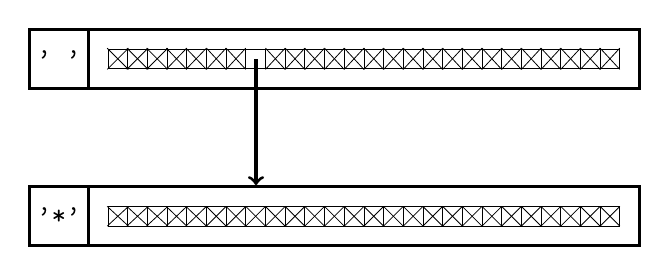
\begin{tikzpicture}

\draw (0.125, 0.125)
  node[draw, line width=0.01cm, , color=black,
       rounded corners=0cm, inner sep=0cm] {

\begin{minipage}[t][0.25cm]{0.25cm}
\mbox{}

\end{minipage}

};
\draw (0.375, 0.125)
  node[draw, line width=0.01cm, , color=black,
       rounded corners=0cm, inner sep=0cm] {

\begin{minipage}[t][0.25cm]{0.25cm}
\mbox{}

\end{minipage}

};
\draw (0.625, 0.125)
  node[draw, line width=0.01cm, , color=black,
       rounded corners=0cm, inner sep=0cm] {

\begin{minipage}[t][0.25cm]{0.25cm}
\mbox{}

\end{minipage}

};
\draw (0.875, 0.125)
  node[draw, line width=0.01cm, , color=black,
       rounded corners=0cm, inner sep=0cm] {

\begin{minipage}[t][0.25cm]{0.25cm}
\mbox{}

\end{minipage}

};
\draw (1.125, 0.125)
  node[draw, line width=0.01cm, , color=black,
       rounded corners=0cm, inner sep=0cm] {

\begin{minipage}[t][0.25cm]{0.25cm}
\mbox{}

\end{minipage}

};
\draw (1.375, 0.125)
  node[draw, line width=0.01cm, , color=black,
       rounded corners=0cm, inner sep=0cm] {

\begin{minipage}[t][0.25cm]{0.25cm}
\mbox{}

\end{minipage}

};
\draw (1.625, 0.125)
  node[draw, line width=0.01cm, , color=black,
       rounded corners=0cm, inner sep=0cm] {

\begin{minipage}[t][0.25cm]{0.25cm}
\mbox{}

\end{minipage}

};
\draw (1.875, 0.125)
  node[draw, line width=0.01cm, , color=black,
       rounded corners=0cm, inner sep=0cm] {

\begin{minipage}[t][0.25cm]{0.25cm}
\mbox{}

\end{minipage}

};
\draw (2.125, 0.125)
  node[draw, line width=0.01cm, , color=black,
       rounded corners=0cm, inner sep=0cm] {

\begin{minipage}[t][0.25cm]{0.25cm}
\mbox{}

\end{minipage}

};
\draw (2.375, 0.125)
  node[draw, line width=0.01cm, , color=black,
       rounded corners=0cm, inner sep=0cm] {

\begin{minipage}[t][0.25cm]{0.25cm}
\mbox{}

\end{minipage}

};
\draw (2.625, 0.125)
  node[draw, line width=0.01cm, , color=black,
       rounded corners=0cm, inner sep=0cm] {

\begin{minipage}[t][0.25cm]{0.25cm}
\mbox{}

\end{minipage}

};
\draw (2.875, 0.125)
  node[draw, line width=0.01cm, , color=black,
       rounded corners=0cm, inner sep=0cm] {

\begin{minipage}[t][0.25cm]{0.25cm}
\mbox{}

\end{minipage}

};
\draw (3.125, 0.125)
  node[draw, line width=0.01cm, , color=black,
       rounded corners=0cm, inner sep=0cm] {

\begin{minipage}[t][0.25cm]{0.25cm}
\mbox{}

\end{minipage}

};
\draw (3.375, 0.125)
  node[draw, line width=0.01cm, , color=black,
       rounded corners=0cm, inner sep=0cm] {

\begin{minipage}[t][0.25cm]{0.25cm}
\mbox{}

\end{minipage}

};
\draw (3.625, 0.125)
  node[draw, line width=0.01cm, , color=black,
       rounded corners=0cm, inner sep=0cm] {

\begin{minipage}[t][0.25cm]{0.25cm}
\mbox{}

\end{minipage}

};
\draw (3.875, 0.125)
  node[draw, line width=0.01cm, , color=black,
       rounded corners=0cm, inner sep=0cm] {

\begin{minipage}[t][0.25cm]{0.25cm}
\mbox{}

\end{minipage}

};
\draw (4.125, 0.125)
  node[draw, line width=0.01cm, , color=black,
       rounded corners=0cm, inner sep=0cm] {

\begin{minipage}[t][0.25cm]{0.25cm}
\mbox{}

\end{minipage}

};
\draw (4.375, 0.125)
  node[draw, line width=0.01cm, , color=black,
       rounded corners=0cm, inner sep=0cm] {

\begin{minipage}[t][0.25cm]{0.25cm}
\mbox{}

\end{minipage}

};
\draw (4.625, 0.125)
  node[draw, line width=0.01cm, , color=black,
       rounded corners=0cm, inner sep=0cm] {

\begin{minipage}[t][0.25cm]{0.25cm}
\mbox{}

\end{minipage}

};
\draw (4.875, 0.125)
  node[draw, line width=0.01cm, , color=black,
       rounded corners=0cm, inner sep=0cm] {

\begin{minipage}[t][0.25cm]{0.25cm}
\mbox{}

\end{minipage}

};
\draw (5.125, 0.125)
  node[draw, line width=0.01cm, , color=black,
       rounded corners=0cm, inner sep=0cm] {

\begin{minipage}[t][0.25cm]{0.25cm}
\mbox{}

\end{minipage}

};
\draw (5.375, 0.125)
  node[draw, line width=0.01cm, , color=black,
       rounded corners=0cm, inner sep=0cm] {

\begin{minipage}[t][0.25cm]{0.25cm}
\mbox{}

\end{minipage}

};
\draw (5.625, 0.125)
  node[draw, line width=0.01cm, , color=black,
       rounded corners=0cm, inner sep=0cm] {

\begin{minipage}[t][0.25cm]{0.25cm}
\mbox{}

\end{minipage}

};
\draw (5.875, 0.125)
  node[draw, line width=0.01cm, , color=black,
       rounded corners=0cm, inner sep=0cm] {

\begin{minipage}[t][0.25cm]{0.25cm}
\mbox{}

\end{minipage}

};
\draw (6.125, 0.125)
  node[draw, line width=0.01cm, , color=black,
       rounded corners=0cm, inner sep=0cm] {

\begin{minipage}[t][0.25cm]{0.25cm}
\mbox{}

\end{minipage}

};
\draw (6.375, 0.125)
  node[draw, line width=0.01cm, , color=black,
       rounded corners=0cm, inner sep=0cm] {

\begin{minipage}[t][0.25cm]{0.25cm}
\mbox{}

\end{minipage}

};
\draw (3.25, 0.125)
  node[draw, line width=0.04cm, , color=black,
       rounded corners=0cm, inner sep=0cm] {

\begin{minipage}[t][0.75cm]{7.0cm}
\mbox{}

\end{minipage}

};\draw[line width=0.01cm,black] (-0.01,0.26) to  (0.26,-0.01);
\draw[line width=0.01cm,black] (0.26,0.26) to  (-0.01,-0.01);
\draw[line width=0.01cm,black] (0.24,0.26) to  (0.51,-0.01);
\draw[line width=0.01cm,black] (0.51,0.26) to  (0.24,-0.01);
\draw[line width=0.01cm,black] (0.49,0.26) to  (0.76,-0.01);
\draw[line width=0.01cm,black] (0.76,0.26) to  (0.49,-0.01);
\draw[line width=0.01cm,black] (0.74,0.26) to  (1.0,-0.01);
\draw[line width=0.01cm,black] (1.0,0.26) to  (0.74,-0.01);
\draw[line width=0.01cm,black] (0.99,0.26) to  (1.25,-0.01);
\draw[line width=0.01cm,black] (1.25,0.26) to  (0.99,-0.01);
\draw[line width=0.01cm,black] (1.25,0.26) to  (1.5,-0.01);
\draw[line width=0.01cm,black] (1.5,0.26) to  (1.25,-0.01);
\draw[line width=0.01cm,black] (1.5,0.26) to  (1.75,-0.01);
\draw[line width=0.01cm,black] (1.75,0.26) to  (1.5,-0.01);
\draw[line width=0.01cm,black] (2.0,0.26) to  (2.25,-0.01);
\draw[line width=0.01cm,black] (2.25,0.26) to  (2.0,-0.01);
\draw[line width=0.01cm,black] (2.25,0.26) to  (2.5,-0.01);
\draw[line width=0.01cm,black] (2.5,0.26) to  (2.25,-0.01);
\draw[line width=0.01cm,black] (2.5,0.26) to  (2.75,-0.01);
\draw[line width=0.01cm,black] (2.75,0.26) to  (2.5,-0.01);
\draw[line width=0.01cm,black] (2.75,0.26) to  (3.0,-0.01);
\draw[line width=0.01cm,black] (3.0,0.26) to  (2.75,-0.01);
\draw[line width=0.01cm,black] (3.0,0.26) to  (3.25,-0.01);
\draw[line width=0.01cm,black] (3.25,0.26) to  (3.0,-0.01);
\draw[line width=0.01cm,black] (3.25,0.26) to  (3.5,-0.01);
\draw[line width=0.01cm,black] (3.5,0.26) to  (3.25,-0.01);
\draw[line width=0.01cm,black] (3.5,0.26) to  (3.75,-0.01);
\draw[line width=0.01cm,black] (3.75,0.26) to  (3.5,-0.01);
\draw[line width=0.01cm,black] (3.75,0.26) to  (4.0,-0.01);
\draw[line width=0.01cm,black] (4.0,0.26) to  (3.75,-0.01);
\draw[line width=0.01cm,black] (4.0,0.26) to  (4.25,-0.01);
\draw[line width=0.01cm,black] (4.25,0.26) to  (4.0,-0.01);
\draw[line width=0.01cm,black] (4.25,0.26) to  (4.5,-0.01);
\draw[line width=0.01cm,black] (4.5,0.26) to  (4.25,-0.01);
\draw[line width=0.01cm,black] (4.5,0.26) to  (4.75,-0.01);
\draw[line width=0.01cm,black] (4.75,0.26) to  (4.5,-0.01);
\draw[line width=0.01cm,black] (4.75,0.26) to  (5.0,-0.01);
\draw[line width=0.01cm,black] (5.0,0.26) to  (4.75,-0.01);
\draw[line width=0.01cm,black] (5.0,0.26) to  (5.25,-0.01);
\draw[line width=0.01cm,black] (5.25,0.26) to  (5.0,-0.01);
\draw[line width=0.01cm,black] (5.25,0.26) to  (5.5,-0.01);
\draw[line width=0.01cm,black] (5.5,0.26) to  (5.25,-0.01);
\draw[line width=0.01cm,black] (5.5,0.26) to  (5.75,-0.01);
\draw[line width=0.01cm,black] (5.75,0.26) to  (5.5,-0.01);
\draw[line width=0.01cm,black] (5.75,0.26) to  (6.0,-0.01);
\draw[line width=0.01cm,black] (6.0,0.26) to  (5.75,-0.01);
\draw[line width=0.01cm,black] (6.0,0.26) to  (6.25,-0.01);
\draw[line width=0.01cm,black] (6.25,0.26) to  (6.0,-0.01);
\draw[line width=0.01cm,black] (6.25,0.26) to  (6.5,-0.01);
\draw[line width=0.01cm,black] (6.5,0.26) to  (6.25,-0.01);

\draw (-0.625, 0.125)
  node[draw, line width=0.04cm, , color=black,
       rounded corners=0cm, inner sep=0cm] {

\begin{minipage}[t][0.75cm]{0.75cm}
\mbox{}

\end{minipage}

};\draw (-0.625, 0.125) node[color=black] {\texttt{' '}};
\draw (0.125, -1.875)
  node[draw, line width=0.01cm, , color=black,
       rounded corners=0cm, inner sep=0cm] {

\begin{minipage}[t][0.25cm]{0.25cm}
\mbox{}

\end{minipage}

};
\draw (0.375, -1.875)
  node[draw, line width=0.01cm, , color=black,
       rounded corners=0cm, inner sep=0cm] {

\begin{minipage}[t][0.25cm]{0.25cm}
\mbox{}

\end{minipage}

};
\draw (0.625, -1.875)
  node[draw, line width=0.01cm, , color=black,
       rounded corners=0cm, inner sep=0cm] {

\begin{minipage}[t][0.25cm]{0.25cm}
\mbox{}

\end{minipage}

};
\draw (0.875, -1.875)
  node[draw, line width=0.01cm, , color=black,
       rounded corners=0cm, inner sep=0cm] {

\begin{minipage}[t][0.25cm]{0.25cm}
\mbox{}

\end{minipage}

};
\draw (1.125, -1.875)
  node[draw, line width=0.01cm, , color=black,
       rounded corners=0cm, inner sep=0cm] {

\begin{minipage}[t][0.25cm]{0.25cm}
\mbox{}

\end{minipage}

};
\draw (1.375, -1.875)
  node[draw, line width=0.01cm, , color=black,
       rounded corners=0cm, inner sep=0cm] {

\begin{minipage}[t][0.25cm]{0.25cm}
\mbox{}

\end{minipage}

};
\draw (1.625, -1.875)
  node[draw, line width=0.01cm, , color=black,
       rounded corners=0cm, inner sep=0cm] {

\begin{minipage}[t][0.25cm]{0.25cm}
\mbox{}

\end{minipage}

};
\draw (1.875, -1.875)
  node[draw, line width=0.01cm, , color=black,
       rounded corners=0cm, inner sep=0cm] {

\begin{minipage}[t][0.25cm]{0.25cm}
\mbox{}

\end{minipage}

};
\draw (2.125, -1.875)
  node[draw, line width=0.01cm, , color=black,
       rounded corners=0cm, inner sep=0cm] {

\begin{minipage}[t][0.25cm]{0.25cm}
\mbox{}

\end{minipage}

};
\draw (2.375, -1.875)
  node[draw, line width=0.01cm, , color=black,
       rounded corners=0cm, inner sep=0cm] {

\begin{minipage}[t][0.25cm]{0.25cm}
\mbox{}

\end{minipage}

};
\draw (2.625, -1.875)
  node[draw, line width=0.01cm, , color=black,
       rounded corners=0cm, inner sep=0cm] {

\begin{minipage}[t][0.25cm]{0.25cm}
\mbox{}

\end{minipage}

};
\draw (2.875, -1.875)
  node[draw, line width=0.01cm, , color=black,
       rounded corners=0cm, inner sep=0cm] {

\begin{minipage}[t][0.25cm]{0.25cm}
\mbox{}

\end{minipage}

};
\draw (3.125, -1.875)
  node[draw, line width=0.01cm, , color=black,
       rounded corners=0cm, inner sep=0cm] {

\begin{minipage}[t][0.25cm]{0.25cm}
\mbox{}

\end{minipage}

};
\draw (3.375, -1.875)
  node[draw, line width=0.01cm, , color=black,
       rounded corners=0cm, inner sep=0cm] {

\begin{minipage}[t][0.25cm]{0.25cm}
\mbox{}

\end{minipage}

};
\draw (3.625, -1.875)
  node[draw, line width=0.01cm, , color=black,
       rounded corners=0cm, inner sep=0cm] {

\begin{minipage}[t][0.25cm]{0.25cm}
\mbox{}

\end{minipage}

};
\draw (3.875, -1.875)
  node[draw, line width=0.01cm, , color=black,
       rounded corners=0cm, inner sep=0cm] {

\begin{minipage}[t][0.25cm]{0.25cm}
\mbox{}

\end{minipage}

};
\draw (4.125, -1.875)
  node[draw, line width=0.01cm, , color=black,
       rounded corners=0cm, inner sep=0cm] {

\begin{minipage}[t][0.25cm]{0.25cm}
\mbox{}

\end{minipage}

};
\draw (4.375, -1.875)
  node[draw, line width=0.01cm, , color=black,
       rounded corners=0cm, inner sep=0cm] {

\begin{minipage}[t][0.25cm]{0.25cm}
\mbox{}

\end{minipage}

};
\draw (4.625, -1.875)
  node[draw, line width=0.01cm, , color=black,
       rounded corners=0cm, inner sep=0cm] {

\begin{minipage}[t][0.25cm]{0.25cm}
\mbox{}

\end{minipage}

};
\draw (4.875, -1.875)
  node[draw, line width=0.01cm, , color=black,
       rounded corners=0cm, inner sep=0cm] {

\begin{minipage}[t][0.25cm]{0.25cm}
\mbox{}

\end{minipage}

};
\draw (5.125, -1.875)
  node[draw, line width=0.01cm, , color=black,
       rounded corners=0cm, inner sep=0cm] {

\begin{minipage}[t][0.25cm]{0.25cm}
\mbox{}

\end{minipage}

};
\draw (5.375, -1.875)
  node[draw, line width=0.01cm, , color=black,
       rounded corners=0cm, inner sep=0cm] {

\begin{minipage}[t][0.25cm]{0.25cm}
\mbox{}

\end{minipage}

};
\draw (5.625, -1.875)
  node[draw, line width=0.01cm, , color=black,
       rounded corners=0cm, inner sep=0cm] {

\begin{minipage}[t][0.25cm]{0.25cm}
\mbox{}

\end{minipage}

};
\draw (5.875, -1.875)
  node[draw, line width=0.01cm, , color=black,
       rounded corners=0cm, inner sep=0cm] {

\begin{minipage}[t][0.25cm]{0.25cm}
\mbox{}

\end{minipage}

};
\draw (6.125, -1.875)
  node[draw, line width=0.01cm, , color=black,
       rounded corners=0cm, inner sep=0cm] {

\begin{minipage}[t][0.25cm]{0.25cm}
\mbox{}

\end{minipage}

};
\draw (6.375, -1.875)
  node[draw, line width=0.01cm, , color=black,
       rounded corners=0cm, inner sep=0cm] {

\begin{minipage}[t][0.25cm]{0.25cm}
\mbox{}

\end{minipage}

};
\draw (3.25, -1.875)
  node[draw, line width=0.04cm, , color=black,
       rounded corners=0cm, inner sep=0cm] {

\begin{minipage}[t][0.75cm]{7.0cm}
\mbox{}

\end{minipage}

};\draw[line width=0.01cm,black] (-0.01,-1.75) to  (0.26,-2.0);
\draw[line width=0.01cm,black] (0.26,-1.75) to  (-0.01,-2.0);
\draw[line width=0.01cm,black] (0.24,-1.75) to  (0.51,-2.0);
\draw[line width=0.01cm,black] (0.51,-1.75) to  (0.24,-2.0);
\draw[line width=0.01cm,black] (0.49,-1.75) to  (0.76,-2.0);
\draw[line width=0.01cm,black] (0.76,-1.75) to  (0.49,-2.0);
\draw[line width=0.01cm,black] (0.74,-1.75) to  (1.0,-2.0);
\draw[line width=0.01cm,black] (1.0,-1.75) to  (0.74,-2.0);
\draw[line width=0.01cm,black] (0.99,-1.75) to  (1.25,-2.0);
\draw[line width=0.01cm,black] (1.25,-1.75) to  (0.99,-2.0);
\draw[line width=0.01cm,black] (1.25,-1.75) to  (1.5,-2.0);
\draw[line width=0.01cm,black] (1.5,-1.75) to  (1.25,-2.0);
\draw[line width=0.01cm,black] (1.5,-1.75) to  (1.75,-2.0);
\draw[line width=0.01cm,black] (1.75,-1.75) to  (1.5,-2.0);
\draw[line width=0.01cm,black] (1.75,-1.75) to  (2.0,-2.0);
\draw[line width=0.01cm,black] (2.0,-1.75) to  (1.75,-2.0);
\draw[line width=0.01cm,black] (2.0,-1.75) to  (2.25,-2.0);
\draw[line width=0.01cm,black] (2.25,-1.75) to  (2.0,-2.0);
\draw[line width=0.01cm,black] (2.25,-1.75) to  (2.5,-2.0);
\draw[line width=0.01cm,black] (2.5,-1.75) to  (2.25,-2.0);
\draw[line width=0.01cm,black] (2.5,-1.75) to  (2.75,-2.0);
\draw[line width=0.01cm,black] (2.75,-1.75) to  (2.5,-2.0);
\draw[line width=0.01cm,black] (2.75,-1.75) to  (3.0,-2.0);
\draw[line width=0.01cm,black] (3.0,-1.75) to  (2.75,-2.0);
\draw[line width=0.01cm,black] (3.0,-1.75) to  (3.25,-2.0);
\draw[line width=0.01cm,black] (3.25,-1.75) to  (3.0,-2.0);
\draw[line width=0.01cm,black] (3.25,-1.75) to  (3.5,-2.0);
\draw[line width=0.01cm,black] (3.5,-1.75) to  (3.25,-2.0);
\draw[line width=0.01cm,black] (3.5,-1.75) to  (3.75,-2.0);
\draw[line width=0.01cm,black] (3.75,-1.75) to  (3.5,-2.0);
\draw[line width=0.01cm,black] (3.75,-1.75) to  (4.0,-2.0);
\draw[line width=0.01cm,black] (4.0,-1.75) to  (3.75,-2.0);
\draw[line width=0.01cm,black] (4.0,-1.75) to  (4.25,-2.0);
\draw[line width=0.01cm,black] (4.25,-1.75) to  (4.0,-2.0);
\draw[line width=0.01cm,black] (4.25,-1.75) to  (4.5,-2.0);
\draw[line width=0.01cm,black] (4.5,-1.75) to  (4.25,-2.0);
\draw[line width=0.01cm,black] (4.5,-1.75) to  (4.75,-2.0);
\draw[line width=0.01cm,black] (4.75,-1.75) to  (4.5,-2.0);
\draw[line width=0.01cm,black] (4.75,-1.75) to  (5.0,-2.0);
\draw[line width=0.01cm,black] (5.0,-1.75) to  (4.75,-2.0);
\draw[line width=0.01cm,black] (5.0,-1.75) to  (5.25,-2.0);
\draw[line width=0.01cm,black] (5.25,-1.75) to  (5.0,-2.0);
\draw[line width=0.01cm,black] (5.25,-1.75) to  (5.5,-2.0);
\draw[line width=0.01cm,black] (5.5,-1.75) to  (5.25,-2.0);
\draw[line width=0.01cm,black] (5.5,-1.75) to  (5.75,-2.0);
\draw[line width=0.01cm,black] (5.75,-1.75) to  (5.5,-2.0);
\draw[line width=0.01cm,black] (5.75,-1.75) to  (6.0,-2.0);
\draw[line width=0.01cm,black] (6.0,-1.75) to  (5.75,-2.0);
\draw[line width=0.01cm,black] (6.0,-1.75) to  (6.25,-2.0);
\draw[line width=0.01cm,black] (6.25,-1.75) to  (6.0,-2.0);
\draw[line width=0.01cm,black] (6.25,-1.75) to  (6.5,-2.0);
\draw[line width=0.01cm,black] (6.5,-1.75) to  (6.25,-2.0);

\draw (-0.625, -1.875)
  node[draw, line width=0.04cm, , color=black,
       rounded corners=0cm, inner sep=0cm] {

\begin{minipage}[t][0.75cm]{0.75cm}
\mbox{}

\end{minipage}

};\draw (-0.625, -1.875) node[color=black] {\texttt{'*'}};\draw[line width=0.04cm,black,->] (1.88,0.12) to  (1.88,-1.48);
\end{tikzpicture}

\end{center}


This NFA accepts 
\[
L(a^* \cup bba)
= L(a)^* \cup L(bba)
\]
Now using the Kleene star construction, we get
\begin{console}[frame=single,fontsize=\footnotesize]
[student@localhost stack] g++ main.cpp; ./a.out
42 42
2 2
0 0
5 5
1 1
0 0
\end{console}


which accepts
\[
L((a^* \cup bba)^*) = L(a^* \cup bba)^*
\]
Let me simplify this a little before we continue.
First I do this:

\begin{center}

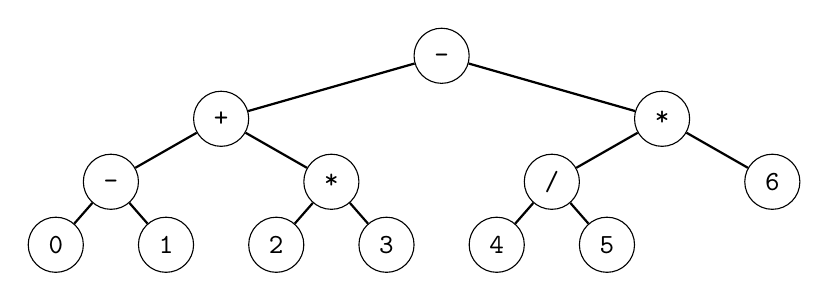
\begin{tikzpicture}
\node at (4.8999999999999995,-0.8) [circle,draw,minimum size=7mm] (A) {\texttt{-}};
\node at (2.0999999999999996,-1.6) [circle,draw,minimum size=7mm] (B) {\texttt{+}};
\node at (7.699999999999999,-1.6) [circle,draw,minimum size=7mm] (C) {\texttt{*}};
\node at (0.7,-2.4000000000000004) [circle,draw,minimum size=7mm] (D) {\texttt{-}};
\node at (3.5,-2.4000000000000004) [circle,draw,minimum size=7mm] (E) {\texttt{*}};
\node at (6.3,-2.4000000000000004) [circle,draw,minimum size=7mm] (F) {\texttt{/}};
\node at (9.1,-2.4000000000000004) [circle,draw,minimum size=7mm] (G) {\texttt{6}};
\node at (0.0,-3.2) [circle,draw,minimum size=7mm] (H) {\texttt{0}};
\node at (1.4,-3.2) [circle,draw,minimum size=7mm] (I) {\texttt{1}};
\node at (2.8,-3.2) [circle,draw,minimum size=7mm] (J) {\texttt{2}};
\node at (4.199999999999999,-3.2) [circle,draw,minimum size=7mm] (K) {\texttt{3}};
\node at (5.6,-3.2) [circle,draw,minimum size=7mm] (L) {\texttt{4}};
\node at (7.0,-3.2) [circle,draw,minimum size=7mm] (M) {\texttt{5}};
\draw [-,thick] (A) -- (B);
\draw [-,thick] (A) -- (C);
\draw [-,thick] (B) -- (D);
\draw [-,thick] (B) -- (E);
\draw [-,thick] (C) -- (F);
\draw [-,thick] (C) -- (G);
\draw [-,thick] (D) -- (H);
\draw [-,thick] (D) -- (I);
\draw [-,thick] (E) -- (J);
\draw [-,thick] (E) -- (K);
\draw [-,thick] (F) -- (L);
\draw [-,thick] (F) -- (M);

;
\end{tikzpicture}
    
\end{center}


then this:
\begin{center}
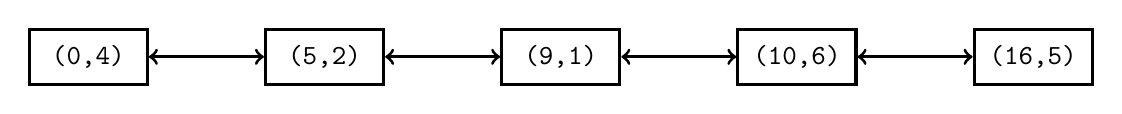
\begin{tikzpicture}

\draw (0.75, 0.35)
  node[draw, line width=0.04cm, , color=black,
       rounded corners=0cm, inner sep=0cm] {

\begin{minipage}[t][0.7cm]{1.5cm}
\mbox{}

\end{minipage}

};\draw (0.75, 0.35) node[color=black] {{\texttt{(0,4)}}};
\draw (3.75, 0.35)
  node[draw, line width=0.04cm, , color=black,
       rounded corners=0cm, inner sep=0cm] {

\begin{minipage}[t][0.7cm]{1.5cm}
\mbox{}

\end{minipage}

};\draw (3.75, 0.35) node[color=black] {{\texttt{(5,2)}}};
\draw (6.75, 0.35)
  node[draw, line width=0.04cm, , color=black,
       rounded corners=0cm, inner sep=0cm] {

\begin{minipage}[t][0.7cm]{1.5cm}
\mbox{}

\end{minipage}

};\draw (6.75, 0.35) node[color=black] {{\texttt{(9,1)}}};
\draw (9.75, 0.35)
  node[draw, line width=0.04cm, , color=black,
       rounded corners=0cm, inner sep=0cm] {

\begin{minipage}[t][0.7cm]{1.5cm}
\mbox{}

\end{minipage}

};\draw (9.75, 0.35) node[color=black] {{\texttt{(10,6)}}};
\draw (12.75, 0.35)
  node[draw, line width=0.04cm, , color=black,
       rounded corners=0cm, inner sep=0cm] {

\begin{minipage}[t][0.7cm]{1.5cm}
\mbox{}

\end{minipage}

};\draw (12.75, 0.35) node[color=black] {{\texttt{(16,5)}}};\draw[line width=0.04cm,black,<->] (1.52,0.35) to  (2.98,0.35);
\draw[line width=0.04cm,black,<->] (4.52,0.35) to  (5.98,0.35);
\draw[line width=0.04cm,black,<->] (7.52,0.35) to  (8.98,0.35);
\draw[line width=0.04cm,black,<->] (10.52,0.35) to  (11.98,0.35);
\end{tikzpicture}

\end{center}


and then this:
\begin{center}
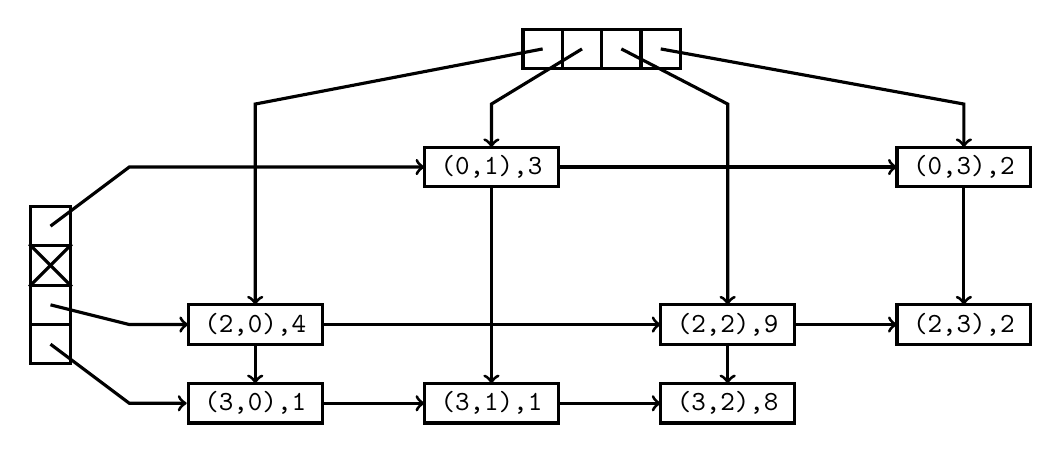
\begin{tikzpicture}

\draw (3.8499999999999996, 3.25)
  node[draw, line width=0.04cm, , color=black,
       rounded corners=0cm, inner sep=0cm] {

\begin{minipage}[t][0.5cm]{1.7cm}
\mbox{}

\end{minipage}

};\draw (3.8499999999999996, 3.25) node[color=black] {{\texttt{(0,1),3}}};
\draw (9.85, 3.25)
  node[draw, line width=0.04cm, , color=black,
       rounded corners=0cm, inner sep=0cm] {

\begin{minipage}[t][0.5cm]{1.7cm}
\mbox{}

\end{minipage}

};\draw (9.85, 3.25) node[color=black] {{\texttt{(0,3),2}}};
\draw (0.85, 1.25)
  node[draw, line width=0.04cm, , color=black,
       rounded corners=0cm, inner sep=0cm] {

\begin{minipage}[t][0.5cm]{1.7cm}
\mbox{}

\end{minipage}

};\draw (0.85, 1.25) node[color=black] {{\texttt{(2,0),4}}};
\draw (6.85, 1.25)
  node[draw, line width=0.04cm, , color=black,
       rounded corners=0cm, inner sep=0cm] {

\begin{minipage}[t][0.5cm]{1.7cm}
\mbox{}

\end{minipage}

};\draw (6.85, 1.25) node[color=black] {{\texttt{(2,2),9}}};
\draw (9.85, 1.25)
  node[draw, line width=0.04cm, , color=black,
       rounded corners=0cm, inner sep=0cm] {

\begin{minipage}[t][0.5cm]{1.7cm}
\mbox{}

\end{minipage}

};\draw (9.85, 1.25) node[color=black] {{\texttt{(2,3),2}}};
\draw (0.85, 0.25)
  node[draw, line width=0.04cm, , color=black,
       rounded corners=0cm, inner sep=0cm] {

\begin{minipage}[t][0.5cm]{1.7cm}
\mbox{}

\end{minipage}

};\draw (0.85, 0.25) node[color=black] {{\texttt{(3,0),1}}};
\draw (3.8499999999999996, 0.25)
  node[draw, line width=0.04cm, , color=black,
       rounded corners=0cm, inner sep=0cm] {

\begin{minipage}[t][0.5cm]{1.7cm}
\mbox{}

\end{minipage}

};\draw (3.8499999999999996, 0.25) node[color=black] {{\texttt{(3,1),1}}};
\draw (6.85, 0.25)
  node[draw, line width=0.04cm, , color=black,
       rounded corners=0cm, inner sep=0cm] {

\begin{minipage}[t][0.5cm]{1.7cm}
\mbox{}

\end{minipage}

};\draw (6.85, 0.25) node[color=black] {{\texttt{(3,2),8}}};\draw[line width=0.04cm,black,->] (4.7,3.25) to  (9,3.25);
\draw[line width=0.04cm,black,->] (7.7,1.25) to  (9,1.25);
\draw[line width=0.04cm,black,->] (1.7,0.25) to  (3,0.25);
\draw[line width=0.04cm,black,->] (4.7,0.25) to  (6,0.25);
\draw[line width=0.04cm,black,->] (3.85,3) to  (3.85,0.5);
\draw[line width=0.04cm,black,->] (6.85,1) to  (6.85,0.5);
\draw[line width=0.04cm,black,->] (9.85,3) to  (9.85,1.5);
\draw[line width=0.04cm,black,->] (1.7,1.25) to  (6,1.25);
\draw[line width=0.04cm,black,->] (0.85,1) to  (0.85,0.5);

\draw (-1.75, 2.5)
  node[draw, line width=0.04cm, , color=black,
       rounded corners=0cm, inner sep=0cm] {

\begin{minipage}[t][0.5cm]{0.5cm}
\mbox{}

\end{minipage}

};
\draw (-1.75, 2.0)
  node[draw, line width=0.04cm, , color=black,
       rounded corners=0cm, inner sep=0cm] {

\begin{minipage}[t][0.5cm]{0.5cm}
\mbox{}

\end{minipage}

};
\draw (-1.75, 1.5)
  node[draw, line width=0.04cm, , color=black,
       rounded corners=0cm, inner sep=0cm] {

\begin{minipage}[t][0.5cm]{0.5cm}
\mbox{}

\end{minipage}

};
\draw (-1.75, 1.0)
  node[draw, line width=0.04cm, , color=black,
       rounded corners=0cm, inner sep=0cm] {

\begin{minipage}[t][0.5cm]{0.5cm}
\mbox{}

\end{minipage}

};\draw[line width=0.04cm,black,->] (-1.75,2.5) to  (-0.75,3.25) to  (3,3.25);
\draw[line width=0.04cm,black] (-2.02,2.27) to  (-1.48,1.73);
\draw[line width=0.04cm,black] (-1.48,2.27) to  (-2.02,1.73);
\draw[line width=0.04cm,black,->] (-1.75,1.5) to  (-0.75,1.25) to  (0,1.25);
\draw[line width=0.04cm,black,->] (-1.75,1.0) to  (-0.75,0.25) to  (-0.02,0.25);

\draw (4.5, 4.75)
  node[draw, line width=0.04cm, , color=black,
       rounded corners=0cm, inner sep=0cm] {

\begin{minipage}[t][0.5cm]{0.5cm}
\mbox{}

\end{minipage}

};
\draw (5.0, 4.75)
  node[draw, line width=0.04cm, , color=black,
       rounded corners=0cm, inner sep=0cm] {

\begin{minipage}[t][0.5cm]{0.5cm}
\mbox{}

\end{minipage}

};
\draw (5.5, 4.75)
  node[draw, line width=0.04cm, , color=black,
       rounded corners=0cm, inner sep=0cm] {

\begin{minipage}[t][0.5cm]{0.5cm}
\mbox{}

\end{minipage}

};
\draw (6.0, 4.75)
  node[draw, line width=0.04cm, , color=black,
       rounded corners=0cm, inner sep=0cm] {

\begin{minipage}[t][0.5cm]{0.5cm}
\mbox{}

\end{minipage}

};\draw[line width=0.04cm,black,->] (4.5,4.75) to  (0.85,4.05) to  (0.85,1.5);
\draw[line width=0.04cm,black,->] (5.0,4.75) to  (3.85,4.05) to  (3.85,3.5);
\draw[line width=0.04cm,black,->] (5.5,4.75) to  (6.85,4.05) to  (6.85,1.5);
\draw[line width=0.04cm,black,->] (6.0,4.75) to  (9.85,4.05) to  (9.85,3.5);
\end{tikzpicture}

\end{center}



Now for 
\[
L((bab \cup ab)^* ) 
= 
L(bab \cup ab)^* 
\]
An NFA accepting this language is

\begin{center}

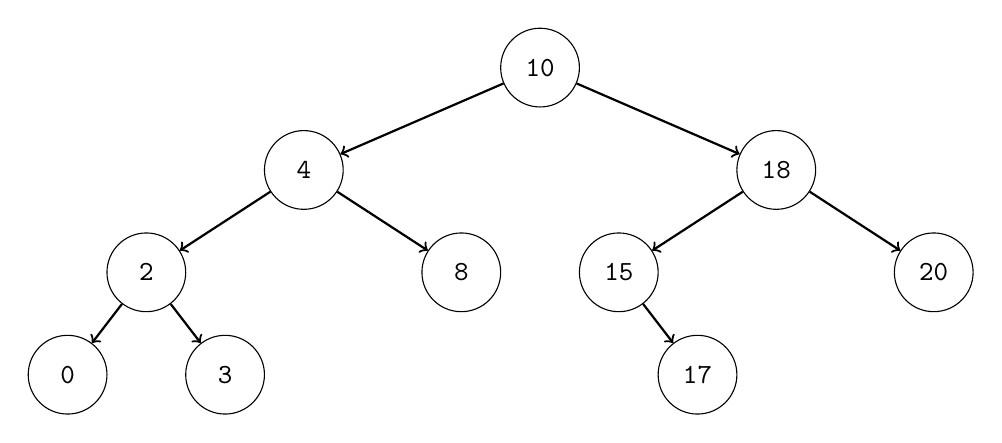
\begin{tikzpicture}
\node at (6,-1.3) [circle,draw,minimum size=10mm] (a) {\texttt{10}};
\node at (3,-2.6) [circle,draw,minimum size=10mm] (b) {\texttt{4}};
\node at (9,-2.6) [circle,draw,minimum size=10mm] (d) {\texttt{18}};
\node at (1,-3.9000000000000004) [circle,draw,minimum size=10mm] (e) {\texttt{2}};
\node at (5,-3.9000000000000004) [circle,draw,minimum size=10mm] (f) {\texttt{8}};
\node at (7,-3.9000000000000004) [circle,draw,minimum size=10mm] (h) {\texttt{15}};
\node at (11,-3.9000000000000004) [circle,draw,minimum size=10mm] (j) {\texttt{20}};
\node at (0,-5.2) [circle,draw,minimum size=10mm] (k) {\texttt{0}};
\node at (2,-5.2) [circle,draw,minimum size=10mm] (l) {\texttt{3}};
\node at (8,-5.2) [circle,draw,minimum size=10mm] (m) {\texttt{17}};
\draw [->,thick] (a) -- (b);
\draw [->,thick] (a) -- (d);
\draw [->,thick] (b) -- (e);
\draw [->,thick] (b) -- (f);
\draw [->,thick] (d) -- (h);
\draw [->,thick] (d) -- (j);
\draw [->,thick] (e) -- (k);
\draw [->,thick] (e) -- (l);
\draw [->,thick] (h) -- (m);

;
\end{tikzpicture}
    
\end{center}


I'm going to simplify it to

\begin{center}
\begin{tikzpicture}[>=triangle 60,shorten >=0.5pt,node distance=2cm,auto,initial text=, double distance=2pt]
\node[state] (A) at (  0,  0) {$0$};
\node[state] (B) at (  3,  0) {$1$};
\node[state] (F) at (  6,  0) {$2$};
\node[state] (C) at (  0, -2) {$3$};
\node[state] (D) at (  3, -2) {$4$};
\node[state] (E) at (  6, -2) {$5$};

\path[->]
(A) edge [loop above] node {} ()
(A) edge [bend left=0,pos=0.5,above] node {} (B)
(B) edge [bend left=0,pos=0.5] node {} (D)
(B) edge [bend left=0,pos=0.5,above] node {} (E)
(C) edge [bend left=0,pos=0.5,above] node {} (B)
(C) edge [bend left=0,pos=0.5,above] node {} (D)
(D) edge [bend left=0,pos=0.5,above] node {} (E)

;
\end{tikzpicture}
\end{center}
    

and then this
\begin{center}
\begin{tikzpicture}

\fill[white] (18.0, -2.0) circle (0.3);
\node [line width=0.03cm,black,minimum size=0.57cm,draw,circle] at (18.0,-2.0)(A){};\draw (18.0, -2.0) node[color=black] {\texttt{20}};
\fill[white] (13.0, 0.0) circle (0.3);
\node [line width=0.03cm,black,minimum size=0.57cm,draw,circle] at (13.0,0.0)(a){};\draw (13.0, 0.0) node[color=black] {\texttt{10}};
\fill[white] (10.0, -1.0) circle (0.3);
\node [line width=0.03cm,black,minimum size=0.57cm,draw,circle] at (10.0,-1.0)(b){};\draw (10.0, -1.0) node[color=black] {\texttt{8}};
\fill[white] (16.0, -1.0) circle (0.3);
\node [line width=0.03cm,black,minimum size=0.57cm,draw,circle] at (16.0,-1.0)(p){};\draw (16.0, -1.0) node[color=black] {\texttt{18}};
\fill[white] (8.0, -2.0) circle (0.3);
\node [line width=0.03cm,black,minimum size=0.57cm,draw,circle] at (8.0,-2.0)(e){};\draw (8.0, -2.0) node[color=black] {\texttt{2}};
\fill[white] (7.0, -3.0) circle (0.3);
\node [line width=0.03cm,black,minimum size=0.57cm,draw,circle] at (7.0,-3.0)(k){};\draw (7.0, -3.0) node[color=black] {\texttt{0}};
\fill[white] (9.0, -3.0) circle (0.3);
\node [line width=0.03cm,black,minimum size=0.57cm,draw,circle] at (9.0,-3.0)(l){};\draw (9.0, -3.0) node[color=black] {\texttt{3}};
\fill[white] (14.0, -2.0) circle (0.3);
\node [line width=0.03cm,black,minimum size=0.57cm,draw,circle] at (14.0,-2.0)(h){};\draw (14.0, -2.0) node[color=black] {\texttt{15}};
\fill[white] (15.0, -3.0) circle (0.3);
\node [line width=0.03cm,black,minimum size=0.57cm,draw,circle] at (15.0,-3.0)(m){};\draw (15.0, -3.0) node[color=black] {\texttt{17}};\draw[line width=0.03cm,black,->,>=triangle 60] (a) to  (p);
\draw[line width=0.03cm,black,->,>=triangle 60] (h) to  (m);
\draw[line width=0.03cm,black,->,>=triangle 60] (a) to  (b);
\draw[line width=0.03cm,black,->,>=triangle 60] (p) to  (h);
\draw[line width=0.03cm,black,->,>=triangle 60] (p) to  (A);
\draw[line width=0.03cm,black,->,>=triangle 60] (b) to  (e);
\draw[line width=0.03cm,black,->,>=triangle 60] (e) to  (k);
\draw[line width=0.03cm,black,->,>=triangle 60] (e) to  (l);
\end{tikzpicture}

\end{center}


And finally when I concat the two machines I get

\begin{center}
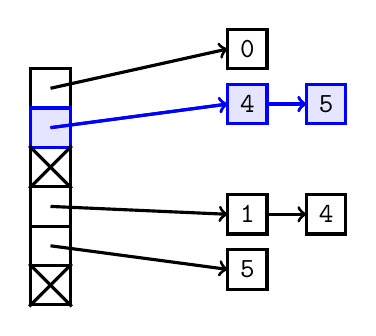
\begin{tikzpicture}

\draw (0.25, -0.25)
  node[draw, line width=0.04cm, , color=black,
       rounded corners=0cm, inner sep=0cm] {

\begin{minipage}[t][0.5cm]{0.5cm}
\mbox{}

\end{minipage}

};
\draw (0.25, -0.75)
  node[fill=blue!10,rounded corners=0cm,inner sep=0cm] {

\begin{minipage}[t][0.5cm]{0.5cm}
\mbox{}

\end{minipage}

};
\draw (0.25, -0.75)
  node[draw, line width=0.04cm, , color=blue,
       rounded corners=0cm, inner sep=0cm] {

\begin{minipage}[t][0.5cm]{0.5cm}
\mbox{}

\end{minipage}

};
\draw (0.25, -1.25)
  node[draw, line width=0.04cm, , color=black,
       rounded corners=0cm, inner sep=0cm] {

\begin{minipage}[t][0.5cm]{0.5cm}
\mbox{}

\end{minipage}

};
\draw (0.25, -1.75)
  node[draw, line width=0.04cm, , color=black,
       rounded corners=0cm, inner sep=0cm] {

\begin{minipage}[t][0.5cm]{0.5cm}
\mbox{}

\end{minipage}

};
\draw (0.25, -2.25)
  node[draw, line width=0.04cm, , color=black,
       rounded corners=0cm, inner sep=0cm] {

\begin{minipage}[t][0.5cm]{0.5cm}
\mbox{}

\end{minipage}

};
\draw (0.25, -2.75)
  node[draw, line width=0.04cm, , color=black,
       rounded corners=0cm, inner sep=0cm] {

\begin{minipage}[t][0.5cm]{0.5cm}
\mbox{}

\end{minipage}

};
\draw (0.25, -0.75)
  node[fill=blue!10,rounded corners=0cm,inner sep=0cm] {

\begin{minipage}[t][0.5cm]{0.5cm}
\mbox{}

\end{minipage}

};
\draw (0.25, -0.75)
  node[draw, line width=0.04cm, , color=blue,
       rounded corners=0cm, inner sep=0cm] {

\begin{minipage}[t][0.5cm]{0.5cm}
\mbox{}

\end{minipage}

};\draw[line width=0.04cm,black] (-0.02,-0.98) to  (0.52,-1.52);
\draw[line width=0.04cm,black] (0.52,-0.98) to  (-0.02,-1.52);
\draw[line width=0.04cm,black] (-0.02,-2.48) to  (0.52,-3.02);
\draw[line width=0.04cm,black] (0.52,-2.48) to  (-0.02,-3.02);

\draw (2.75, 0.24999999999999992)
  node[draw, line width=0.04cm, , color=black,
       rounded corners=0cm, inner sep=0cm] {

\begin{minipage}[t][0.5cm]{0.5cm}
\mbox{}

\end{minipage}

};\draw (2.75, 0.24999999999999992) node[color=black] {{\texttt{0}}};
\draw (2.75, -0.45000000000000007)
  node[fill=blue!10,rounded corners=0cm,inner sep=0cm] {

\begin{minipage}[t][0.5cm]{0.5cm}
\mbox{}

\end{minipage}

};
\draw (2.75, -0.45000000000000007)
  node[draw, line width=0.04cm, , color=blue,
       rounded corners=0cm, inner sep=0cm] {

\begin{minipage}[t][0.5cm]{0.5cm}
\mbox{}

\end{minipage}

};\draw (2.75, -0.45000000000000007) node[color=black] {{\texttt{4}}};
\draw (3.75, -0.45000000000000007)
  node[fill=blue!10,rounded corners=0cm,inner sep=0cm] {

\begin{minipage}[t][0.5cm]{0.5cm}
\mbox{}

\end{minipage}

};
\draw (3.75, -0.45000000000000007)
  node[draw, line width=0.04cm, , color=blue,
       rounded corners=0cm, inner sep=0cm] {

\begin{minipage}[t][0.5cm]{0.5cm}
\mbox{}

\end{minipage}

};\draw (3.75, -0.45000000000000007) node[color=black] {{\texttt{5}}};
\draw (2.75, -1.85)
  node[draw, line width=0.04cm, , color=black,
       rounded corners=0cm, inner sep=0cm] {

\begin{minipage}[t][0.5cm]{0.5cm}
\mbox{}

\end{minipage}

};\draw (2.75, -1.85) node[color=black] {{\texttt{1}}};
\draw (3.75, -1.85)
  node[draw, line width=0.04cm, , color=black,
       rounded corners=0cm, inner sep=0cm] {

\begin{minipage}[t][0.5cm]{0.5cm}
\mbox{}

\end{minipage}

};\draw (3.75, -1.85) node[color=black] {{\texttt{4}}};
\draw (2.75, -2.55)
  node[draw, line width=0.04cm, , color=black,
       rounded corners=0cm, inner sep=0cm] {

\begin{minipage}[t][0.5cm]{0.5cm}
\mbox{}

\end{minipage}

};\draw (2.75, -2.55) node[color=black] {{\texttt{5}}};
\draw (2.75, -0.45000000000000007)
  node[fill=blue!10,rounded corners=0cm,inner sep=0cm] {

\begin{minipage}[t][0.5cm]{0.5cm}
\mbox{}

\end{minipage}

};
\draw (2.75, -0.45000000000000007)
  node[draw, line width=0.04cm, , color=blue,
       rounded corners=0cm, inner sep=0cm] {

\begin{minipage}[t][0.5cm]{0.5cm}
\mbox{}

\end{minipage}

};\draw (2.75, -0.45000000000000007) node[color=black] {{\texttt{4}}};
\draw (3.75, -0.45000000000000007)
  node[fill=blue!10,rounded corners=0cm,inner sep=0cm] {

\begin{minipage}[t][0.5cm]{0.5cm}
\mbox{}

\end{minipage}

};
\draw (3.75, -0.45000000000000007)
  node[draw, line width=0.04cm, , color=blue,
       rounded corners=0cm, inner sep=0cm] {

\begin{minipage}[t][0.5cm]{0.5cm}
\mbox{}

\end{minipage}

};\draw (3.75, -0.45000000000000007) node[color=black] {{\texttt{5}}};\draw[line width=0.04cm,black,->] (0.25,-0.25) to  (2.5,0.25);
\draw[line width=0.04cm,blue,->] (0.25,-0.75) to  (2.5,-0.45);
\draw[line width=0.04cm,blue,->] (3.0,-0.45) to  (3.5,-0.45);
\draw[line width=0.04cm,black,->] (0.25,-1.75) to  (2.5,-1.85);
\draw[line width=0.04cm,black,->] (3.0,-1.85) to  (3.5,-1.85);
\draw[line width=0.04cm,black,->] (0.25,-2.25) to  (2.5,-2.55);
\draw[line width=0.04cm,blue,->] (0.25,-0.75) to  (2.5,-0.45);
\draw[line width=0.04cm,blue,->] (3.0,-0.45) to  (3.5,-0.45);
\end{tikzpicture}

\end{center}




\begin{ex} 
  \label{ex:some-decision1}
  \tinysidebar{\debug{exercises/{empty0/question.tex}}}
  \solutionlink{sol:some-decision1}
  \qed
\end{ex} 
\begin{python0}
from solutions import *
add(label="ex:some-decision1",
    srcfilename='exercises/some-decision1/answer.tex') 
\end{python0}


\newpage
The big picture is this:
Regular expressions are constructed starting from the symbols in $\Sigma$
or $\emptyset$
(and you know how to construct NFAs for all these).
You combine regular expressions recursively using
unions, concatenation, and Kleene star (and you know how to 
construct the unions, concatenations, and Kleene stars of NFAs).
Therefore the languages accepted by regex must be contained in the 
languages accepted by NFAs.

That's the main idea.

Formally, the right strategy is to proof the following statement
\begin{enumerate}
\item[]
If $r$ is a regular expression, then there is an NFA $N$
such that $L(N) = L(r)$.
\end{enumerate}
by mathematical induction on the length of the regex 
(remember: a regex is a string.)
In other words you should form this:
\begin{enumerate}
\item[]
$P(n)$: If $r$ is a regular expression of length $n$, 
then there is an NFA $N$
such that $L(N) = L(r)$.
\end{enumerate}

You then prove this by induction.
The base case starts at $n = 1$ since a regex have at least one character.
The base cases are 
\[
r = c
\]
where $c \in \Sigma$ or
\[
r = \emptyset
\]
It's easy to construct NFAs for these regex (of course!).
So the base case is ... DONE!

Now you assume $P(1), P(2), \ldots, P(n)$ is true for some $n \geq 1$.
Now you want to prove $P(n+1)$, i.e., 
given any regex $r$ of length $n + 1$, you want to 
prove that there is an NFA $N$ such that
\[
L(N) = L(r)
\]
You can of course assume $n \geq 1$ since we're done with the base case.
Now what?

Well, since the length of $r$ is $n + 1 > 1$, $r$ must be either
\[
r = s^*
\]
where $s$ is a regex, or
\[
r = st
\]
where $s$ and $t$ are regexes, or
\[
r = s \cup t
\]
where $s$ and $t$ are regexes.
(For simplicity, I'm ignoring the case where the regex has parenthesis,
i.e., $r$ is $(s)$ -- this is an easy case. So I'll leave that to you.)
By definition, there are no other cases.
Note that in the first case the length of $s$ is $\leq n$ (in fact
exactly equal to $n$).
In the second case, the lengths of $s$ and $t$ are both $\leq n$.
Likewise in the third case, the lengths of $s$ and $t$ are both $\leq n$.
By induction hypothesis, for all cases, the $s$ or the $t$
(depending on the cases) are accepted by some NFAs $N_1$ and $N_2$.

In the first case,
since 
\[
L(N_1) = L(s)
\]
we have by definition
\[
L(N_1)^* = L(s)^* = L(s^*)
\]
We also know that the Kleene star operator is a closed operator.
Since $L(N_1)$ is a regular language, this means that 
$L(N_1)^*$ is also regular.
This means that there is some NFA/DFA $N_1'$ such that
\[
L(N_1') = L(N_1)^*
\]
Altogether we have found some NFA/DFA $N_1'$ such that
\[
L(N_1') = L(N_1)^* = L(s^*) = L(r)
\]
We have proven $P(n+1)$ for this case.
All other cases are similar. 
(Go over the proof yourself.)

Therefore $P(n+1)$ is true for all cases.

By mathematical induction, $P(n)$ is true for all $n \geq 1$.

